\documentclass[12pt]{article}
\usepackage[utf8]{inputenc}
\usepackage[frenchb]{babel}
\usepackage[T1]{fontenc}
\usepackage{authblk}
\usepackage{hyperref}
\usepackage{fancyhdr}
\usepackage{titling}
\usepackage{graphicx}
\usepackage{geometry}
\usepackage{enumitem}
\usepackage{microtype}
\usepackage[none]{hyphenat}
%\usepackage[toc]{glossaries}
%\makeglossaries
\usepackage{wrapfig}

\usepackage{perpage} %the perpage package
\MakePerPage{footnote} %the perpage package command

%\newacronym{REST}{REST}{transfert d'état représentationnel}


 \geometry{
 a4paper,
 total={169mm,240mm},
 left=16mm,
 top=20mm,
 }

\usepackage{listings} % For code coloration
\usepackage{color}
\usepackage[dvipsnames]{xcolor}


\definecolor{codegreen}{rgb}{0,0.6,0}
\definecolor{codegray}{rgb}{0.5,0.5,0.5}
\definecolor{codepurple}{rgb}{0.58,0,0.82}
\definecolor{backcolour}{rgb}{0.95,0.95,0.92}


\headheight = 15pt

\hypersetup{colorlinks = true,citecolor=black,filecolor=black,linkcolor=black,urlcolor=black}

\lstdefinestyle{s}{
  backgroundcolor=\color{backcolour},   commentstyle=\color{codegreen},
  keywordstyle=\color{NavyBlue},
  numberstyle=\tiny\color{codegray},
  stringstyle=\color{codepurple},
  basicstyle=\footnotesize,
  breakatwhitespace=false,
  breaklines=true,
  captionpos=b,
  keepspaces=true,
  numbers=left,
  numbersep=5pt,
  showspaces=false,
  showstringspaces=false,
  showtabs=false,
  tabsize=4
}


\lstset{style=s}
\lstset{literate=
  {á}{{\'a}}1 {é}{{\'e}}1 {í}{{\'i}}1 {ó}{{\'o}}1 {ú}{{\'u}}1
  {Á}{{\'A}}1 {É}{{\'E}}1 {Í}{{\'I}}1 {Ó}{{\'O}}1 {Ú}{{\'U}}1
  {à}{{\`a}}1 {è}{{\`e}}1 {ì}{{\`i}}1 {ò}{{\`o}}1 {ù}{{\`u}}1
  {À}{{\`A}}1 {È}{{\'E}}1 {Ì}{{\`I}}1 {Ò}{{\`O}}1 {Ù}{{\`U}}1
  {ä}{{\"a}}1 {ë}{{\"e}}1 {ï}{{\"i}}1 {ö}{{\"o}}1 {ü}{{\"u}}1
  {Ä}{{\"A}}1 {Ë}{{\"E}}1 {Ï}{{\"I}}1 {Ö}{{\"O}}1 {Ü}{{\"U}}1
  {â}{{\^a}}1 {ê}{{\^e}}1 {î}{{\^i}}1 {ô}{{\^o}}1 {û}{{\^u}}1
  {Â}{{\^A}}1 {Ê}{{\^E}}1 {Î}{{\^I}}1 {Ô}{{\^O}}1 {Û}{{\^U}}1
  {œ}{{\oe}}1 {Œ}{{\OE}}1 {æ}{{\ae}}1 {Æ}{{\AE}}1 {ß}{{\ss}}1
  {ű}{{\H{u}}}1 {Ű}{{\H{U}}}1 {ő}{{\H{o}}}1 {Ő}{{\H{O}}}1
  {ç}{{\c c}}1 {Ç}{{\c C}}1 {ø}{{\o}}1 {å}{{\r a}}1 {Å}{{\r A}}1
  {€}{{\EUR}}1 {£}{{\pounds}}1 {°}{{\no}}1
}

\pretitle{
  \begin{center}
  
\includegraphics[width=60mm,height=31mm]{img/univ.png}
  \qquad \qquad
  
\includegraphics[width=37mm,height=31mm]{img/iutNantes.jpg}\\[\bigskipamount]
}

\posttitle{
 \end{center}
}

\title{Back End marketing conversationnel\\
    \normalsize Technologies web côté serveur}
\date{\today}
\author{Paul Orhon\\
\small LP -- MiAR -- Université de Nantes }

\pagestyle{fancy}
\fancyhf{}
\rhead{Paul Orhon --- \small LP -- MiAR}
\lhead{Marketing conversationnel --- Technologies web côté serveur}
\rfoot{Page \thepage}
\lfoot{INSTITUT UNIVERSITAIRE DE TECHNOLOGIE - NANTES}


\begin{document}

\maketitle%page titre
\begin{figure}[h]
    \centering
    
\includegraphics[]{img/logo.png}
\end{figure}

\clearpage
\tableofcontents

\listoffigures


\clearpage

\section{Projet}
Dans le cadre du module de technologies web côté serveur, il a été demandé de créer une partie du back end d’un marketing conversationnel.
\\

Pour cela il va falloir développer différent services pour pouvoirs mettre en place ce système.



\section{Contexte du projet}
\subsection{Objectifs}
L'objectif est donc de développer une partie du Back End d’un marketing conversationnel, en exposant les services avec une api REST.
\\

\begin{figure}[h]
    \centering
    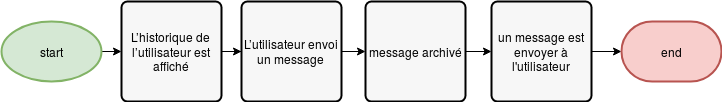
\includegraphics[width=\linewidth]{img/workflow_user.png}
    \caption{Workflow classique d'un utilisateur}
\end{figure}

La partie à développer est l'envoi des messages et les sauvegardes des données. Ces sauvegardes sont utilisées pour conserver les messages, qui seront datés, afin d'afficher l'historique à l'utilisateur et pouvoir effectuer des statistiques anonyme sur toute les conversations.
\\

Le projet doit être séparé en sous module, cela permettra de manipuler, modifier et diffuser plus facilement.


\subsection{Contraintes}
\begin{enumerate}
    \item Le projet est à réalisé seul.
    \item Le programme sera développé sur la plateforme Java.
    \begin{itemize}
        \item Il sera programmé en Java pour des raisons de connaissance.
    \end{itemize}
    \item Le rapport est à rendre le 27 novembre 2017 à 08h00.
    \item Le projet est à rendre le 5 décembre 2017 à 12h20.
    \item Le système doit sauvegarder les messages pour réaliser des statistiques et pour l'historique des utilisateurs.
    \item Le système doit être testé et testable sur le poste du développeur.
    \item Le couplage doit être lâche.
\end{enumerate}


\clearpage
\section{Les vues}
\subsection{Vue globale du projet}

\begin{figure}[h]
    \centering
    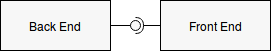
\includegraphics[]{img/Diagramme_sep_Back_Front.png}
    \caption{Diagramme de la séparation du Back / Front End}
    \label{fig:diag_back_front}
\end{figure}
Comme dit précédemment, seule le back end et son interface sera développé (partie en rouge de la figure \ref{fig:diag_back_front}).


\subsection{Vue logique du Back End}
Le back end sera divisé en plusieurs modules permettent ainsi de diviser les tâches, de réaliser un couplage lâche et de faciliter le maintien du système.

Cette représentation repose sur le \textit{domain-driven design}\footnote{\textit{domain-driven design}(DDD): en français \textit{conception pilotée par le domaine} est une approche de la conception de logiciel. Plus d'information: \url{https://en.wikipedia.org/wiki/Domain-driven_design}}. Le but du DDD est de former le code autour de notion métiers.

\begin{figure}[h]
    \centering
    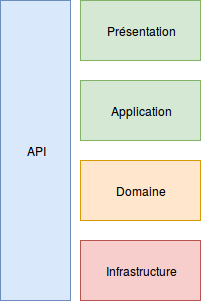
\includegraphics[]{img/Vue_logique_back.png}
    \caption{Diagramme de la vue logique du back end}
\end{figure}

Ici chaque couleur correspond à un module.


\begin{description}
    \item [Application] contient la \textbf{présentation} du fait de l'utilisation du framework \textit{Spring} qui permet une mise en place simple d'une api REST et donc de l'interface du back end. Sont rôle est de récupérer les requête arrivant à l'interface, de les envoyer au bon service et de répondre.
    \item [Domaine] correspond au \textit{services} de l'application. Contient aussi les \textbf{\textit{interfaces}}, pressant  dans l'\textbf{API} et implémenté dans l'\textbf{infrastructure}, utile à ces services.
    \item [Infrastructure] correspond à l'implémentation des différentes \textbf{\textit{interfaces}} et \textbf{\textit{classe abstraites}} qui sont les factory. Il gère le stockage persistant des données.
    \item [API] contient les \textbf{\textit{classe}} communes aux modules. Cela permet notamment au \textbf{domaine} d'utiliser une classe et de laisser l'implémentation à l'\textbf{Infrastructure}.
\end{description}

\section{Implémentation}

\subsection{Les Services}
Le back end va donc proposer différant services.

\subsubsection{L'envoi de messages}
Un service proposera au client d'envoyer un message vers le serveur.
Ce message sera transmis aux personnes concerner. Il sera aussi sauvegardé. Cette sauvegarde est utile pour l'historique de conversation de l'utilisateur (cf. \ref{recup_histo}) et pour réaliser des statistiques sur l'ensemble des demande.


\subsubsection{L'envoi de réponse}
Suite à l'envoi d'un message par un utilisateur, s'il le peut, le serveur envoie un message sinon la personne concernée répond à la demande.\\
Pour le moment le serveur répondra avec un message générique, pour cause d'un manque de temps et de moyen.


\subsubsection{Récupérer l'historique} \label{recup_histo}
L'or de sa connexion l'utilisateur peut récupérer son historique de conversation afin de reprend le fil de sa conversation.
\\
Si l'utilisateur n'a pas d'historique une liste vide lui est retourné.


% \subsection{Plateforme / Langage}

\subsection{Java}
Comme dit précédemment le programme sera développé pour la plateforme java et développer en java et plus précisément dans la version 8. Cela permet de faciliter le déploiement du programme vu que java est multi-plateforme.


\subsection{Librairie}

\subsubsection{Slf4j}
\textit{Slf4j}\footnote{\url{http://www.slf4j.org}} est une api de logging. Elle permet de loger les informations souhaiter à l'endroit souhaiter. Par exemple dans un fichier. Cela va permettre de pouvoir avoir les logs même après l'arrêt du programme, car les messages ne sont plus directement dans le terminal.

\subsubsection{Spring Boot} \label{SpringBoot}
Nous allons aussi utiliser \textit{Spring Boot}\footnote{\url{http://projects.spring.io/spring-boot}} en version 1.5.8 qui est un framework permettant de développer une application web avec une gestion simplifiée des différents services mis en place et de leur présentation sous forme de service REST.

\subsubsection{Spring Boot Test}
\textit{Spring Boot Test}\footnote{\url{https://spring.io/guides/gs/spring-boot/\#_add_unit_tests}} est utilisé pour réaliser les tests de l'api REST. Nous l'utiliserons dans la même version que Spring Boot (cf. \ref{SpringBoot}).

\subsubsection{Junit}
Pour les tests plus générales, nous allons utiliser \textit{junit}\footnote{\url{http://junit.org/junit4/}} en version 4.12, qui est un framework de test unitaire.

\subsubsection{Gson}
\textit{Gson}\footnote{\url{https://github.com/google/gson}} est une librairie qui permet de convertir des objets Java en JSON et inversement. Il nous sera utile pour comprendre les informations reçu et de pouvoir en renvoyer.


\subsection{Outils}
Pour ce projet nous utiliserons différant outils qui vont simplifier le développement.


\subsubsection{IntelliJ IDEA}
\textit{IntelliJ IDEA}\footnote{\url{https://www.jetbrains.com/idea/}} est l'IDE java qui est utilisé pour ce projet. Il va permettre de faciliter le développement grâce à ces différentes options.


\subsubsection{Maven}
\textit{Maven}\footnote{\url{http://maven.apache.org/}} est un outil de gestion et d'automatisation de production des projets Java. Il va être utiles pour la séparation du programme en module, la gestion des dépendances et les build.

\subsubsection{MongoDB}
\textit{MongoDB}\footnote{\url{https://www.mongodb.com/what-is-mongodb}} est un système de gestion de base de données orientée documents, il est simple d'utilisation. Il va être utilisé pour sauvegarder les messages des utilisateurs afin de leur retourner leur historique(cf. \ref{recup_histo}).

\subsubsection{GitHub}
\textit{GitHub}\footnote{\url{https://github.com/}} est un service de gestion de développement. Il va être utilisé pour gérer les versions du projet. Cela va aussi permettre le partage des sources sous licence MIT afin de récupérer le retour des utilisateurs et de leur amélioration.

\subsubsection{Travis-ci}
\textit{Travis-ci}\footnote{\url{https://travis-ci.org/}} est un outil d'intégration continue, qui permet d'effectuer les build et les tests sous différent environnement UNIX. Il permet aussi de déployer les build.\\
Il est aussi possible d'utiliser \textit{AppVeyor} pour un environnement Windows.

\subsubsection{Codecov}
\textit{Codecov}\footnote{\url{https://codecov.io/gh}} est un outil permettant de regrouper, fusionner, archiver et comparer des rapports de couverture de code. Cela permet, notamment, de trouver les codes morts.


\section{Conclusion}
Ce projet a donc pour but de développer le back end et l'interface d'un marketing conversationnel. Pour des raisons de temps seuls l'échange de messages et l'historique sera développé. Le projet sera réalisé en java. Le développement se fera autour des tests afin de valider le fonctionnement des différentes méthodes. Les différentes tâches doivent être séparées pour avoir un couplage lâche. Différent outil serons utilisés pour faciliter le développement.

\begin{figure}[h]
    \centering
    
\includegraphics[]{img/logo.png}
    \caption{Logo}
\end{figure}



%\clearpage
%\printglossary[type=\acronymtype, title=Acronymes]

\end{document}
